\documentclass[12pt,a4paper]{article}

\usepackage[margin=2cm]{geometry}
\usepackage{graphicx}
\usepackage{subcaption}
\usepackage{xcolor}
\usepackage{hyperref}
\usepackage{sansmathfonts}
\renewcommand{\familydefault}{\sfdefault}
\hypersetup{colorlinks=true, linkcolor=blue, urlcolor=blue}
\pagenumbering{gobble}

\graphicspath{{figures/}}

\definecolor{accent}{HTML}{2454FF}

\begin{document}

\begin{center}
  {\LARGE \textbf{Teaching a Neural Network to Predict\\[2pt] the Cost of the Future, for Faster MPC}}\\[10pt]
  {\large Alessandro Wegher}\\[4pt]
  {\small \href{https://github.com/alewegher/ORC_with_FP}{github.com/alewegher/ORC\_with\_FP} --- full technical report inside the repo}
\end{center}

\vspace{8pt}
\noindent\textbf{The problem.} Model Predictive Control (MPC) re-plans a robot's motion at every
time step by solving an optimization problem over a short future window. Look further ahead and
the controller behaves more intelligently, but the optimization gets far more expensive to solve
in real time. Look only a little ahead, and the controller becomes short-sighted: locally
reasonable decisions, globally poor outcomes.

\vspace{6pt}
\noindent\textbf{The idea.} Instead of looking far ahead at every step, train a small neural
network offline to predict \emph{``how expensive is it to finish well from here?''} -- the
cost-to-go. Bolt that prediction onto a short-horizon controller as a \emph{terminal cost}, and it
gets a cheap, learned sense of the long-term consequences of its short-term choices, without
paying for a long-horizon solve online.

\vspace{6pt}
\noindent\textbf{Testbed.} A single pendulum (1 joint) and a double pendulum (2 joints), both
fully actuated. For each, three controllers are compared: a short-horizon MPC, a long-horizon MPC
(expensive, near-optimal, the reference), and the same short horizon with the learned terminal
cost added.

\begin{figure}[htbp!]
  \centering
  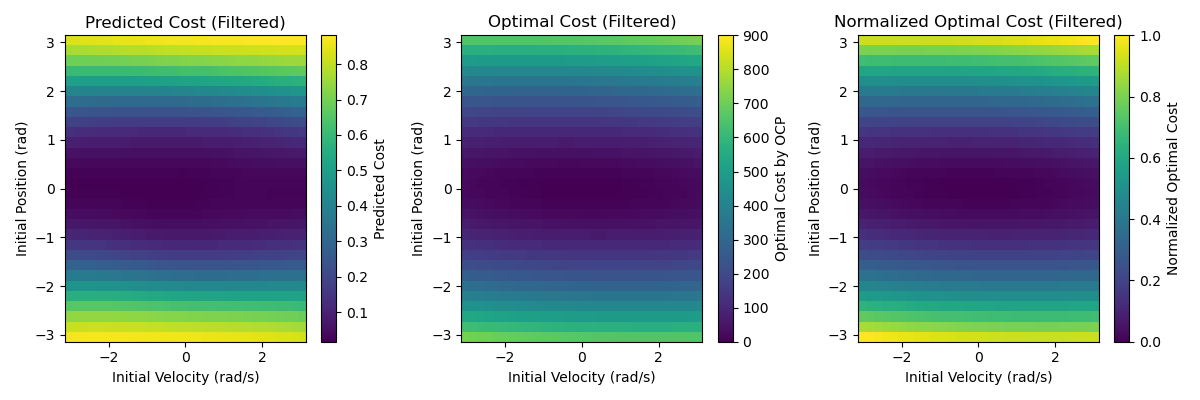
\includegraphics[width=0.62\textwidth]{SP_colormap.png}
  \caption{The network learns to predict cost-to-go directly from a state $(q,\dot q)$ -- brighter
  means a more expensive future. Left: network prediction. Middle: ground truth from solving the
  real optimization problem. Right: ground truth, normalized. The match is close almost
  everywhere.}
\end{figure}

\clearpage

\noindent\textbf{Does it actually work in closed loop?} Predicting the right cost on average
across many starting points is one thing; actually steering a real, running controller the same
way a long-horizon controller would is another. So beyond the aggregate comparison, each
controller was run for real, in receding-horizon closed loop, from the same starting state:

\begin{figure}[htbp!]
  \centering
  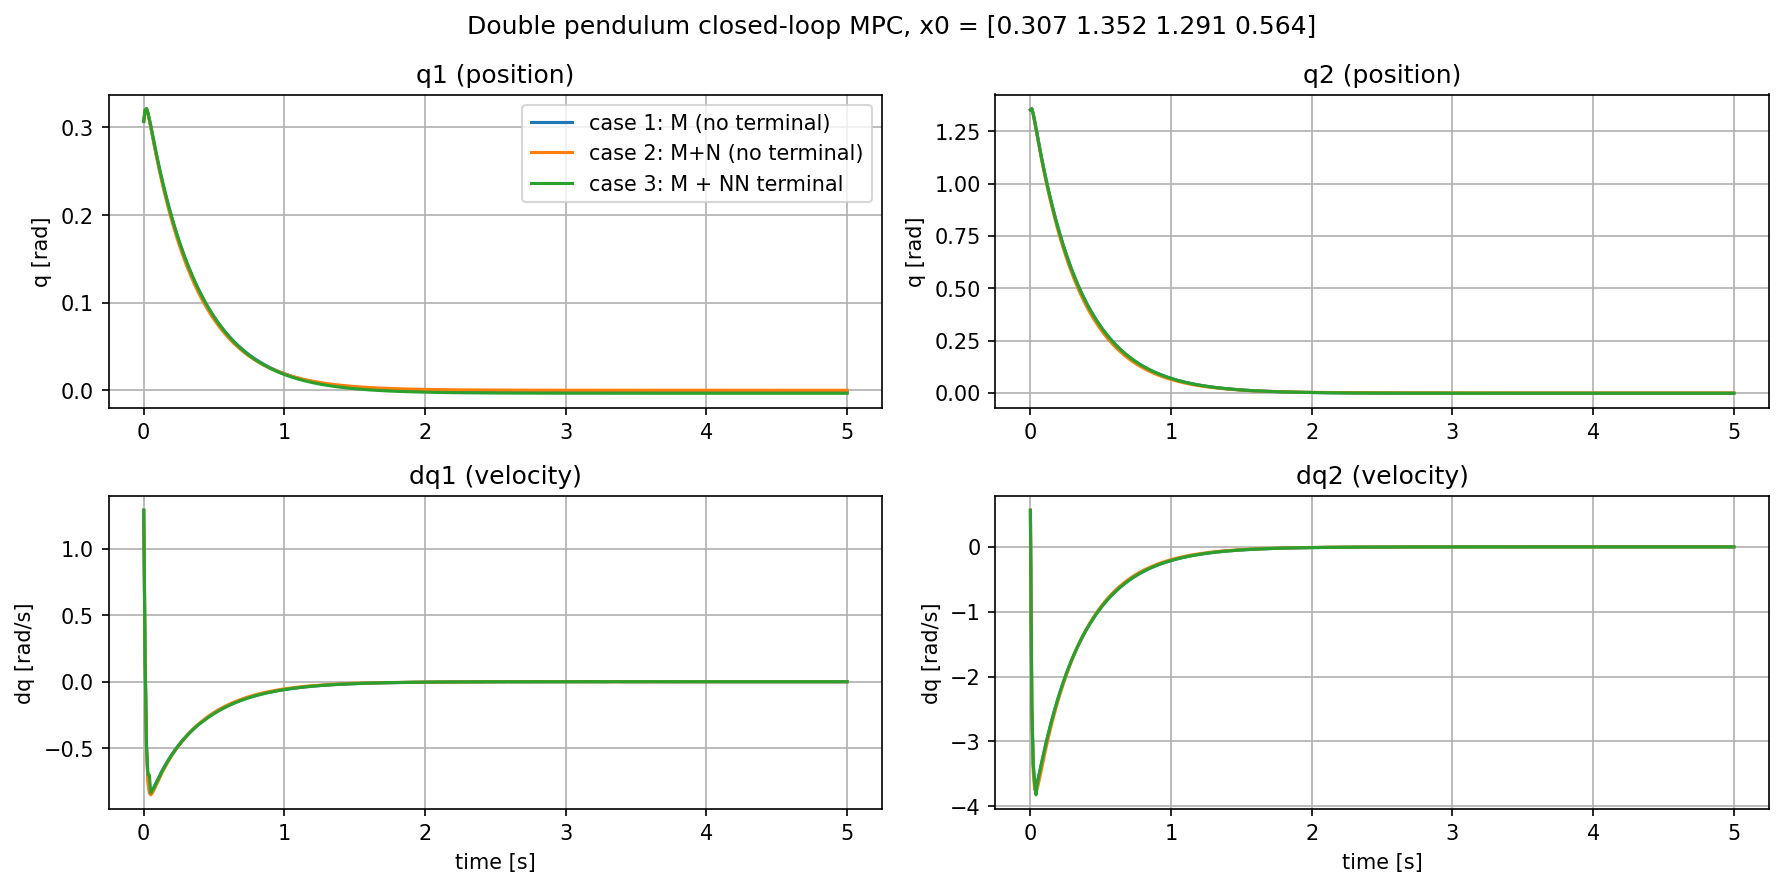
\includegraphics[width=0.85\textwidth]{DP_MPC_traj_kin.png}
  \caption{Double pendulum, closed loop: joint angles and velocities under the three controllers,
  all three curves essentially on top of each other. The short-horizon controller with the
  learned terminal cost matches the expensive long-horizon controller almost exactly --
  \textbf{at 3.5$\times$ less compute} (51.7s vs.\ 178.9s of solver time for this run).}
\end{figure}

\vspace{4pt}
\noindent\textbf{Takeaway.} A cheap, learned terminal cost can recover the benefit of an
expensive long-horizon MPC -- as the double pendulum result above shows, at a fraction of the
compute. But not for free, and not everywhere: on the simpler single-pendulum system, the same
learned terminal cost sometimes fails to pull the short-horizon controller away from its myopic
behaviour, even though it predicts the right cost \emph{on average} across many starting states.
That gap between ``predicts the right value'' and ``actually steers the controller the right
way'' is, to me, the most interesting result here, and a natural next step (matching the value
function's \emph{gradient}, not just its value, during training).

\vspace{10pt}
\noindent {\small Full write-up, all code, and every figure: \href{https://github.com/alewegher/ORC_with_FP}{github.com/alewegher/ORC\_with\_FP}}

\end{document}
